Denne sektion diskuterer det proof of concept der blev lavet til søvn delen af projektet.
Grunden til at der kun laves et proof of concept og ikke et fuldstændigt færdig system er at der er ikke nok tid til at gøre det helt færdigt. 
Ydermere vil et helt færdigt systemet påkræve testning hos målgruppen, og dette er igen en besværlig proces som der ikke er tid nok til at udføre. 

Denne sektion om proof of concept beskriver valg af sensor data som er nødvendigt, hvordan søvnestimering udføres på denne data, og hvordan søvn estimeringerne for de forskellige sensor kombineres og hvordan denne estimeringen skal aggregeres til individuelle perioder af søvn.

% Manglende resourcer
% Time constraints.
% Ingen test mulig(Kræver tilladelser, og system ikke færdig)

Som et proof of concept er der valgt at implementere en enkelt metode til at detektere hvor vidt man sover eller ej.
Metoden der tages udgangspunkt i er den metode som er beskrevet i Best Effort Sleep i \cref{sec:BES}, men andre metoder kunne også have været brugt.
Der vil dog kun tages udgangspunkt i de sensorer der har fået givet en høj koefficient, som kan ses i \cref{tab:vaegtninger}, hvilket gør at amplitude og acceleration er de datakilder der tages udgangspunkt i.
Disse to datakilder kombineres til en enkelt model der skal kunne vurderer hvorvidt man sover.

\subsection{Forsøgsopstilling}
%Disposition:
%Billede af opstilling
%Bare tage med hjem og sove
%Flere forsøg og systematisk tilgang kunne være brugt og skulle gøres hvis det ikke bare var proof of concept.
For at forsøget fortages på ens vis, så det indsamlede data er sammenligneligt valgte vi en forsøgsopstilling.
\begin{figure}[h]
	\centering
	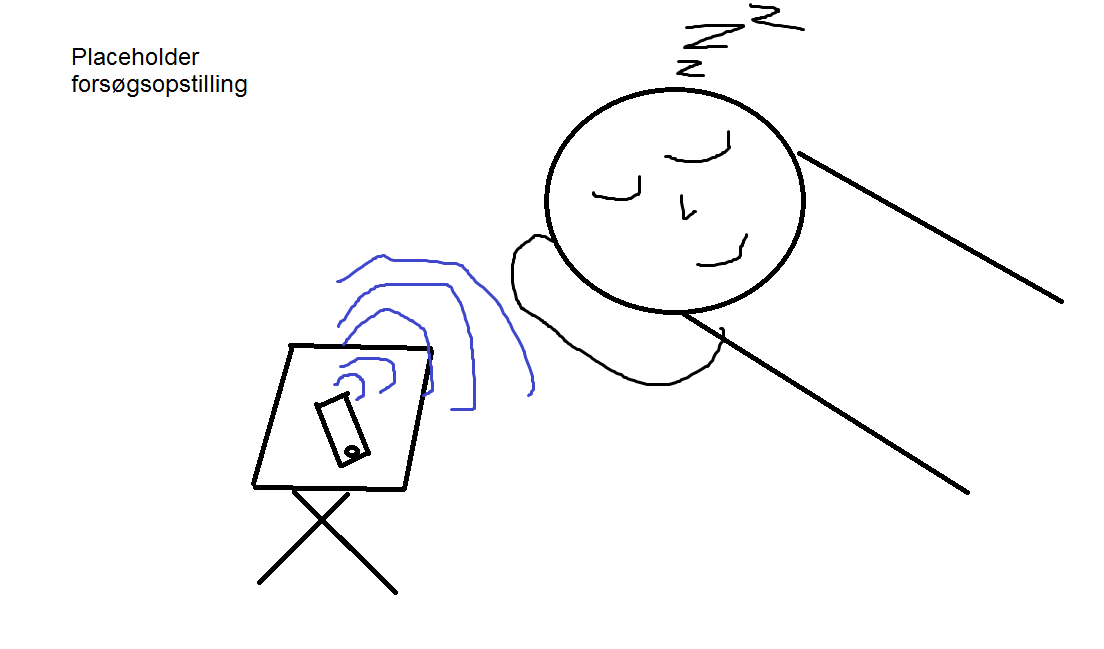
\includegraphics[scale=0.5,trim = 0cm 0cm 5cm 10cm, clip]{forsoegsopstilling}
	\caption{Forsøgsopstilling. Sovende person med telefonen på natbordet.}
	\label{fig:forsoegopstillings}
\end{figure}

Forsøgsopstillingen kan ses i \cref{fig:forsoegopstillings} der illustrerer hvordan telefonen ligger på natbordet og indsamler data.
Idéen er at det eneste krav til indsamlingen er at den skal ligge på et bord i soveværelset når der soves, ellers står det en frit om man går med telefonen i lommen, ligger den på skrivebordet eller andet.

Indsamlingen af data foregik ved at vi installerede de fornødne moduler på egen telefon, og tog telefonen med hjem så data fra en eller flere dage kunne indsamles, hvor vi loggede når vi gik i seng og stod op, hvilket skulle bruges til at afgøre nøjagtigheden af vores estimat.
Da dette er et proof of concept er dette tilstrækkeligt, men hvis man skulle udvikle en bedre egnet model skulle man være mere systematisk, hvor flere testpersoner med forskellige søvnvaner ville blive inddraget og hvor cross-validation eller lignende ville blive benyttet til at verificere ens model.

\subsection{Sensor Data}
Hoved idéen bag brugen af acceleration og amplitude data kan ses i Best Effort Sleep Model i \cref{sec:BES}, men den dækker ikke alle problemscenarier der kan være involveret i brugen af disse data.

For at have en bedre indsigt i hvordan vi kan bruge accelerations og amplitude data blev disse plottet over en dag inklusiv søvn, hvor man holdt log for hvornår der blev sovet.
Dette kan ses i \cref{fig:accplot} og \cref{fig:amplplot}.

\begin{figure}[h]
	\centering
	%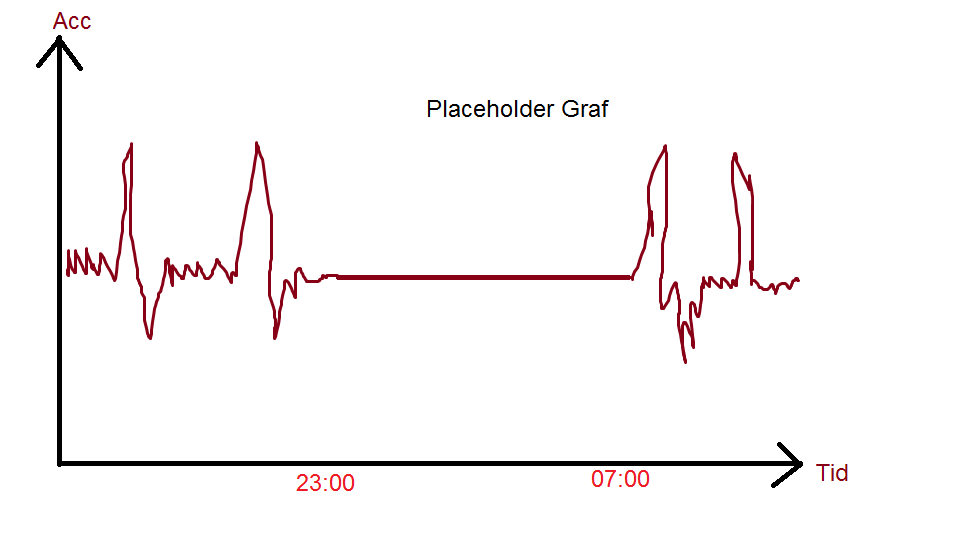
\includegraphics[scale=0.5]{acc-placeholder}
	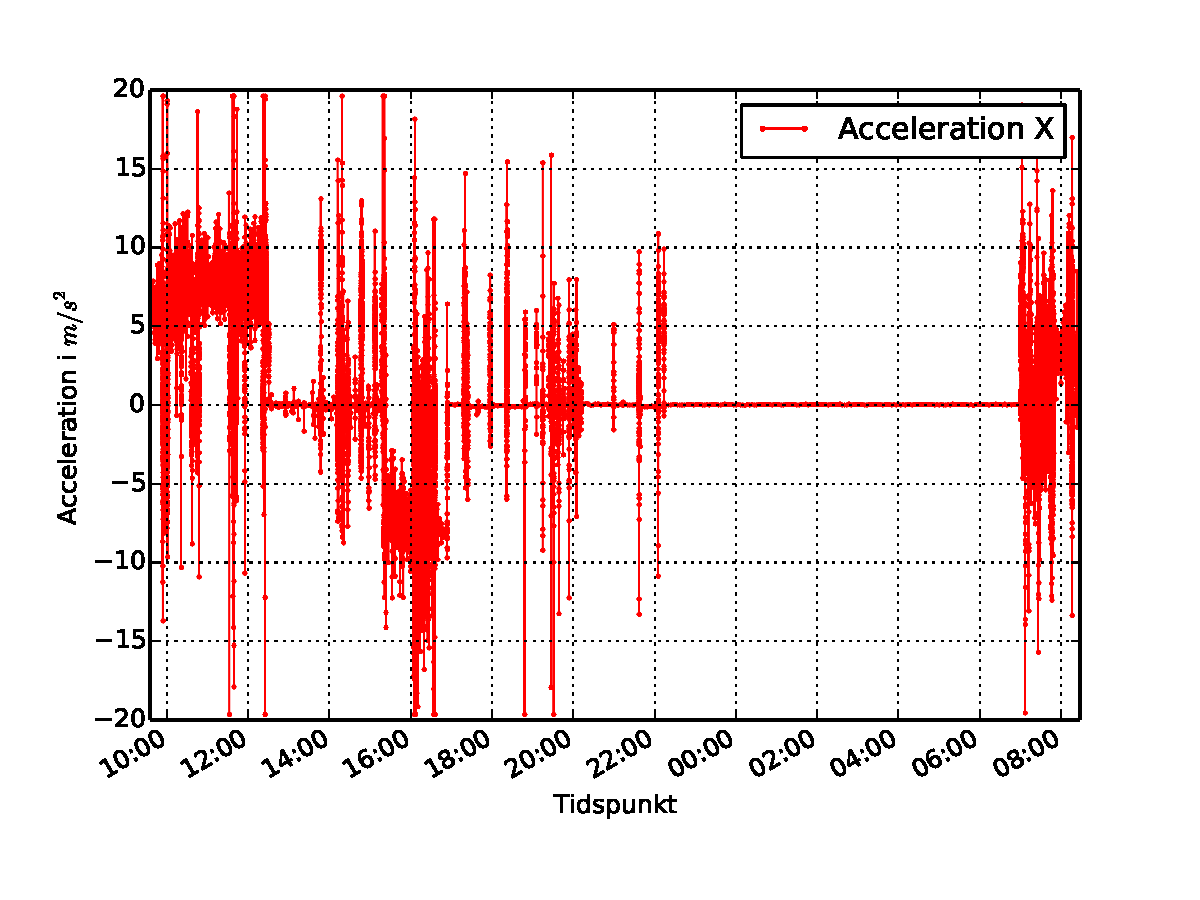
\includegraphics[scale=0.75]{acceleration-plot}
	\caption{Accelerationsplot, hvor der blev sovet fra ca. 22:00 til 07:00 næste dag.  Et punkt svarer til en måleværdi.}\label{fig:accplot}
\end{figure}

Ses der på accelerometer data i \cref{fig:accplot} indikerer det tydeligt når telefonen har været i bevægelse og når telefonen ikke har været i bevægelse.
Dette skyldes at accelerometret er god til at registrere bevægelse, da acceleration er ændring i hastighed.
Det viser sig at plottet fint indikerer når man er vågen, hvilket er forårsaget af at testpersonen har gået med sin telefon i lommen.
Dog kan man ved stilstand ikke vide sig sikker på om det er fordi man sover, eller blot fordi man har lagt sin mobil fra sig.

Ved stilstand i en længere periode kan det forsøges at estimere sandsynligheden for at denne stilstand er grundet at man sover, men derudover kan andre sensor inputs hjælpe til at klargøre denne tvivl, der ikke er begrænset til at man skal have telefonen i lommen.
Et eksempel på en sådan kilde er mikrofonen, som vi kan bruge til at måle maks amplitude, således at man ikke indsamler personfølsomme oplysninger da man ikke kan genskabe en samtale men blot har maks amplitude lagret for hvert sekund.

\begin{figure}[h]
	\centering
	%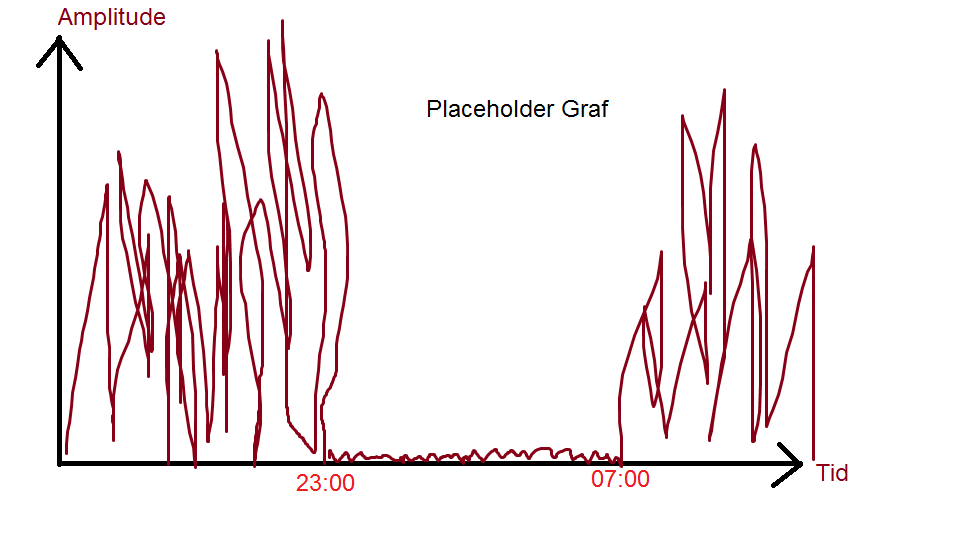
\includegraphics[scale=0.5]{ampl-placeholder}
	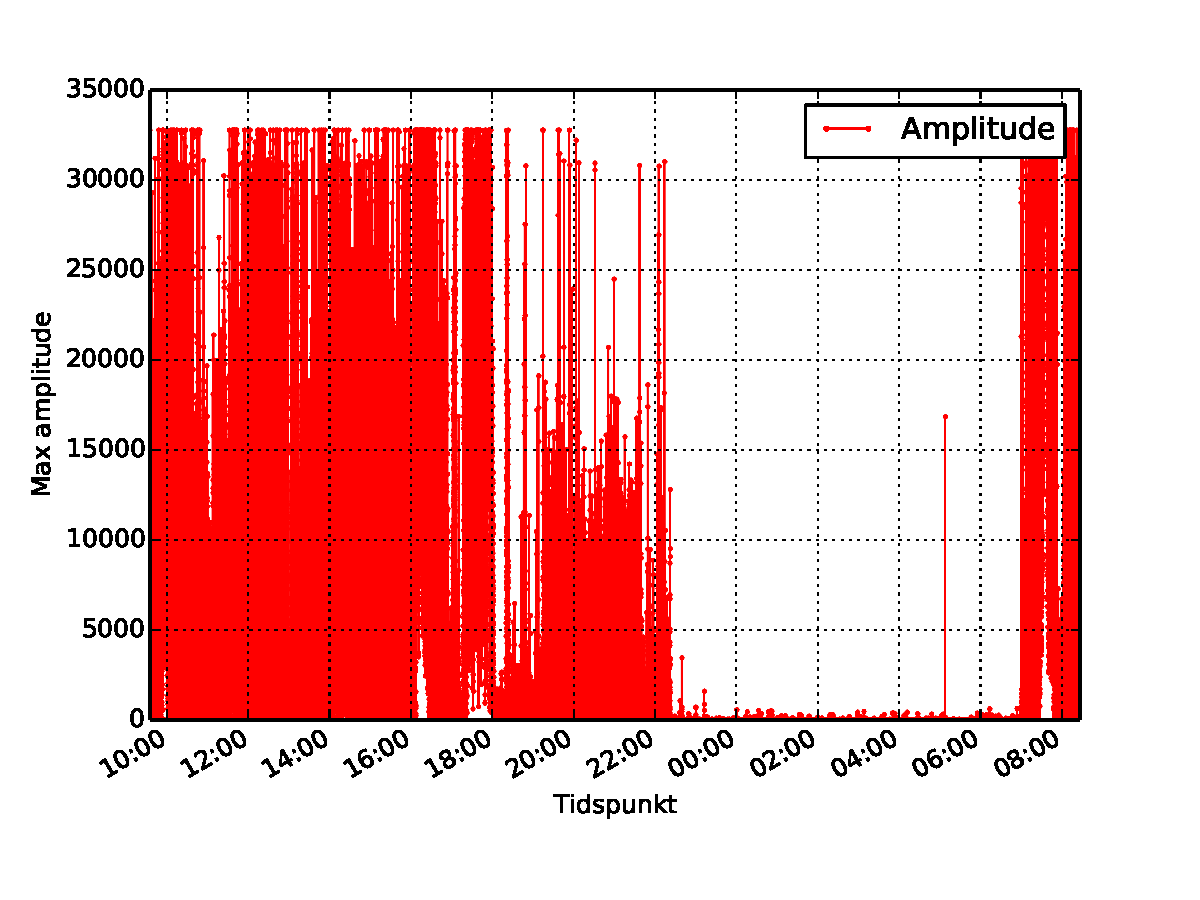
\includegraphics[scale=0.75]{amplitude-plot}
	\caption{Amplitudeplot, hvor der blev sovet fra ca. 22:00 til 07:00 næste dag. Et punkt svarer til en måleværdi.}\label{fig:amplplot}
\end{figure}

Idéen bag at bruge maks amplituden er at man larmer væsentligt mere når man er vågen end når man sover.
Dette passer fint med de loggede data plottet i \cref{fig:amplplot}.
Dog har denne antagelse også begrænsninger.
Eksempelvis kan det være at man er en stille person, snorker meget eller også kunne personen bo i et meget larmende område.
Alligevel regner vi med at amplituden stadig kan bruges, da man så muligvis kunne finde et mønster når man snorker til at styrke modellen, hvilket vil blive diskuteret i \cref{section:snorken}.
Derudover er det så et spørgsmål om hvor stor vægt man skal tillægge de enkelte sensorkilder og er noget der bør trænes til det enkelte individ for at opnå en model der passer til det enkelte individs personlighed.
Hvordan dette gøres bør overvejes ved videreudvikling, men til dette proof of concept kan man som en start bruge fastsatte statiske vægte.

\subsection{Søvnestimerings model}
Ud fra observeret data etablerer vi nogle antagelser som vi går ud fra holder til fremtidigt data også.
Disse er at når man observerer en handling om det er acceleration eller amplitude, kan vi med stor sikkerhed sige at man ikke sover.
Modsat ved stilstand er sandsynligheden for at man sover afhængigt af længden af stilstand.

Dette får os til at lave en model der bygger på disse to antagelser, og er en model der er lavet til at skabe jordforbindelse.
Med dette menes at vi udvikler en metode for at få bekræftigelse på at det kan lade sig gøre at få implementeret til en mobil med den valgte platform.
Vi har ikke kunnet finde passende metoder der er offentligt tilgængeligt, hvorfor vi bliver nødt til at udvikle vores egen algoritme.
Vi tillader os at tage det forbehold at den udviklede model sikkert ikke er en metode der bør anvendes i praksis, men kan alligevel bruges til at udforske nogle af udfordringerne ved søvnestimering.
Nogle af udfordringerne kan sikkert takles med inspiration fra de omtalte metoder som vi vil have i mente, men det er ikke utænkeligt at andre udfordringer dukker op.

Vores model går på en sliding window tilgang hvor den centrale del er at registrere stilstand ved acceleration og amplitude.
\subsubsection{Stilstands Bestemmelse}
Som udgangspunkt for vores udkast til en søvnestimeringsmodel afgøres der hvornår der er stilstand.
Dette gøres forskelligt for acceleration og amplitude data, men tager udgangspunkt i det loggede data.
For at sikre enkelte spikes ikke påvirker resultatet anvendes et vægtet gennemsnit til at reducere støj.

Hvis vi ser på \cref{fig:accplot}, der er et plot for accelerations data kan vi se stilstand for punkterne mellem 22:00 og 07:00.
Øvelsen består i at have en metode der kan afgøre at disse punkter er i stilstand.
Dette gøres ved at for et givent punkt at se om de 5 tidligere målinger ikke afviger fra en given fastsat grænse fra punktet i betragtning i x, y og z aksen.
Pseudokode til at tjekke dette kan ses i \cref{lst:pseudoStationary}.
\begin{lstlisting}[caption={Pseudo kode for at tjekke om et punkt er i stilstand.}, label={lst:pseudoStationary}]
isStationary(accToConsider : AccelerationReading, previousPoints : Collection of AccelerationReadings) : boolean
   foreach acc in previousPoints
      if outOfThreshold(accToConsider, acc)
         return false
   return true
\end{lstlisting}

Hvis der ikke er en sådan afvigelse bestemmes det at punktet i betragtning er i stilstand.
Dette gøres for alle punkter og der afgøres for hvert af disse om de er i stilstand eller ej.
Ved at gøre det på denne måde er man robust overfor påvirkning af tyngdeaccelerationen da denne ville måles konstant hvis telefonen ligger stille.

Ved at betragte amplituden \cref{fig:amplplot} kan her ses stilstand fra lidt over 22:00 til omkring 07:00 med et enkelt spike ved 05:00.
Det enkelte spike takles af det vægtede gennemsnit.
Derudover kan stilstandsbestemmelsen gøres på en måde der ligner den for accelerationen.
Der anvendes altså et sliding window, men i stedet for at se på om de 5 tidligere punkter afviger relativt i.f.t. det givne punkt i betragtning ses der på om de alle ligger under en fastsat tærskel.
At se på 5 tidligere punkter er ikke en fastlagt værdi, men afhænger af samplingsfrekvensen, vi har for amplitude en samplingsfrekvens på 1 måling per sekund så tidshorisonten er på fem sekunder.
At kigge blot fem sekunder tilbage kan være op til debat, og ved videre arbejde er det en parameter man bør justere for at opnå en højere præcision.
Dog holder vi fast i at det er fornuftigt at kigge en tidsperiode tilbage i stedet for en fast mængde punkter.
Dette sikrer at algoritmen også er fremtidssikret m.h.t. til dette, for ellers risikerer vi at nyt hardware har en højere samplingsfrekvens hvor at gå 5 punkter ikke ville fungere, men hvor en tidshorisont ville.


Dermed har vi nogle simple måder at afgøre stilstand på og kan bruges til vores søvnestimering.
\subsubsection{Søvn Estimering}
Resultatet af stilstands bestemmelsen er en række punkter der hver især er klassificeret som stilstand eller ikke stilstand.
Ud fra disse punkter kan der findes perioder med stilstand, og ud fra længden af hver af disse perioder tildeles punkterne en stigende sandsynlighed for søvn alt efter hvor langt fra starten af stilstandsperioden et af de givne punkter i perioden er.


Spørgsmålet går så på hvorledes en funktion skal defineres for en sådan stigende sandsynlighed.
Det skal være en funktion der repræsenterer hvor sikker man er på søvn ud fra længden af stilstand eksempelvis målt i timer.
En sådan funktion bør være lært ud fra ens empiri, så man kunne løse opgaven som et regressionsproblem.
Dette er et område der kan arbejdes videre med for at få en mere akkurat søvnestimeringsmetode og opfordres til at gøres med mere tid.

Dog for at få et udgangspunkt til diskussion af sådanne funktioner er der tre funktioner plottet i \cref{fig:trefunc}.
\begin{figure}[h]
	\centering
	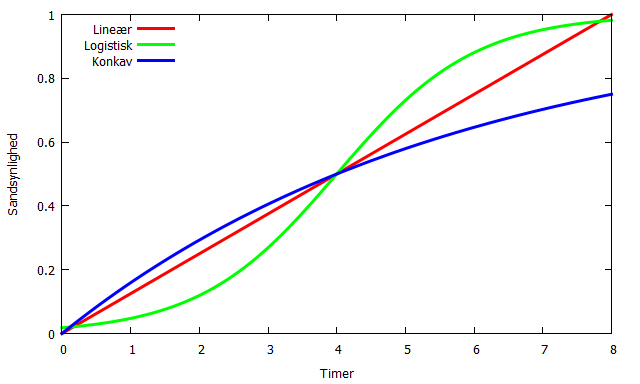
\includegraphics[scale=0.33]{graf-funktionseksempler}
	\caption{Tre funktioner til estimering af sandsynlighed for søvn}\label{fig:trefunc}
\end{figure}

\cref{fig:trefunc} viser tre forslag til en sådan funktion.
Disse er den røde lineære funktion, den blå konkave funktion og den grønne logistiske funktion \citep{wiki:LogisticFunction}.
Alle tre funktioner har til fælles at de er voksende, hvilket passer med vores antagelse af jo længere der har været stilstand jo større sandsynlighed for at man sover.
Den lineære funktion bygger på antagelsen at sandsynligheden for at man sover er kongruent med stilstands længden, hvilket vi ikke ønsker da vi så tillægger for stor vægt til korte stilstandsperioder.
Af samme grund forkastes den konkave funktion også.

Til sidst har vi den logistiske funktion der fint beskriver hvordan at ved længere stilstandsperioden er der en forøget hældning i funktionen indtil vi nærmer os lange stilstandsperioder hvor ekstra tid ikke giver meget ekstra sandsynlighed for søvn men stadig lidt. 
Dette kan ses da den logistiske funktion vi har plottet går asymptotisk mod 1, svarende til 100\% sikkerhed for søvn.
I realiteten kan vi aldrig være 100\% sikker på søvn ved lang stilstand, det kan være man har glemt mobilen hjemme mens man er på tur over en weekend, men hvis forudsætningen for at systemet fungerer er at man har mobilen i nærheden regnes den logistiske funktion som et godt redskab til et søvnestimat.

Definitionen af den logistiske funktion er defineret som følger:
\begin{equation}
	f(t_{span}) = \frac{L}{1+e^{\,-k\cdot(t_{span} - t_{midtpunkt})}}
\end{equation} 
hvor,
\begin{itemize}
	\item[$L$] er kurvens maksimums værdi, hvilket for os eksempelvis kan være $1$ for 100\% sandsynlighed for søvn.
	\item[$k$] er stejlheden for kurven.
	\item[$t_{span}$] Tidsperiode siden starten på stilstandsperioden målt i timer.
	\item[$t_{midtpunkt}$] Er det tidspunkt hvor kurven når $L/2$, hvilket i figurens tilfælde er hvornår kurven når $0.5$ det vil sige ved 4 timer.
\end{itemize}

Der kan argumenteres for en lavere værdi for $L$ så man maks kan blive 90\% sikker, men er noget der bør overvejes med mere træningsdata. Det kan også være en god idé at ændre på stejlheden for kurven, altså k, baseret på hvilken kilde af data man bruger som f.eks. accelerometer eller lyd.

\subsection{Kombinering af modeller}\label{subsec:kombimodeller}
Det er tiltænkt at hver sensor kan have en tilknyttet søvn estimerings model, hvilket i vores tilfælde er en søvn estimerings model for accelerometret og lyd fra mikrofonen.
Imidlertid kan det være en fordel at have en samlet model der kombinerer resultaterne fundet for de enkelte modeller.
En simpel metode at gøre dette på er ved hjælp af et vægtet gennemsnit, hvilket er en metode som \citet{6563918} også benytter.
Det vægtede gennemsnit afviger fra et normalt vægtet gennemsnit da vi har data der ikke er optaget på samme tid og heller ikke data i samme mængder for de enkelte søvnestimerings moduler.
På grund af dette hvis der er en mangel på en estimering til en given tid for et søvn estimerings modul, tages den forrige værdi til estimeringen.
Man kan forestille sig en lynlås hvor der skiftes mellem takkerne fra hver del, ligesom det gøres med estimeringerne for hvert modul.

For at illustrere dette bruges der et eksempel.

\newcommand{\nv}{Ingen estimering}

\begin{table}[h]
\centering
\begin{tabular}{|c|c|c|c|}
\hline Tid & Sandsynlighed for model A & Sandsynlighed for model B & Resultat\\ 
\hline 02:30:00 & 	0.59    & \nv  	& $\text{Vægt}_A * 0.59 + \text{Vægt}_B * 0.29$\\ 
\hline 02:30:01 & 	\nv     & 0.29 	& $\text{Vægt}_A * 0.61 + \text{Vægt}_B * 0.29$\\ 
\hline 02:30:02 & 	0.61    & \nv 	& $\text{Vægt}_A * 0.61 + \text{Vægt}_B * 0.31$\\ 
\hline 02:30:03 & 	0.62    & \nv 	& $\text{Vægt}_A * 0.62 + \text{Vægt}_B * 0.31$\\ 
\hline 02:30:04 & 	\nv     & 0.31 	& ...\\
\hline 
\end{tabular} 
\caption{Tabel der illustrerer hvordan kombineringen fungerer. $\text{Vægt}_A$ og $\text{Vægt}_B$ er de fastsatte vægte for de to modeller.}
\label{tab:combiModelsExample}
\end{table}

I \cref{tab:combiModelsExample} kan man se kombineringen af de to modeller.
Måden den kombinerer sandsynligheder på er ved at den starter med to gennemløbere henholdsvis for A og B som starter på det første element som ikke er tom. 
Så derfor i eksemplet vil A starte ved 02:30:00 med værdien $0.59$ og for B vil den starte ved 02:30:01 med værdien $0.29$. 
Disse to værdier kombineres for det bagerste element med vægtningerne for de to modeller, hvorefter flyttes den bagerste gennemløber, og en ny kombinering foretages.
Dette forsætter indtil der ikke er mere data tilbage i en af de to gennemløbere, hvorefter der ventes på ny data så begge gennemløbere igen har data at køre på.

\subsection{Aggregering}\label{subsec:soevnaggre}
Som demonsteret giver søvnestimeringsmetoden, der er vist som proof of concept, en estimering til en lang række tidspunkter.
Men for at give et ekstra redskab til at danne et overblik over disse estimeringer, kan der med fordel som proof of concept laves en aggregering af søvn estimerings data.

For at få et bedre indblik i formen for data der skal aggregeres gives et eksempel i \cref{tab:noaggsoevndata}.
\begin{table}[h]
	\centering
\begin{tabular}{|c|c|c|}
	\hline {\_}id & prob & time \\ 
	\hline 203754 & 0.050 & 2015-04-26 01:41:42.446 \\ 
	\hline 203755 & 0.050 & 2015-04-25 01:41:43.375 \\ 
	\hline ... & ... & ... \\ 
	\hline 218777 & 0.919 & 2015-04-26 05:52:36.204 \\ 
	\hline 218778 & 0.919 & 2015-04-26 05:52:37.203 \\ 
	\hline 218779 & 0.000 & 2015-04-26 05:52:38.163 \\ 
	\hline 
\end{tabular}
\caption{Eksempel på søvn estimeringsdata der ikke er aggregeret.}\label{tab:noaggsoevndata}
\end{table}
Ved at se på data som i \cref{tab:noaggsoevndata} fremstår det hvordan at fra {\_}id 203754 til {\_}id 218778 er sandsynligheden for søvn, der ses i \textit{prob} kolonnen, monotont voksende.
Idéen derudfra er så at registrere sådanne monotoniforhold og aggregere data med hensyn til det.
Det vil sige at registrere intervaller hvor \textit{prob} er tilpas stor over længere tidsperiode, samt er monotont voksende.

Det blev besluttet at forkaste intervaller kortere end 10 minutter og hvor sandsynligheden for søvn i slutningen af intervallet er under 10\%.
Dette kan være en fornuftig løsning under antagelse af at man er rolig når man sover, og har da også vist gode resultater med nogle tests af personer med en meget rolig søvn. 
Eksempelvis med det viste data i \cref{tab:noaggsoevndata} ville dette blive aggregeret til en række som set i \cref{tab:aggdat}.

\begin{table}[h]
	\centering
\begin{tabular}{|c|c|c|c|}
	\hline {\_}id & startdate & enddate & prob \\ 
	\hline 1 & 2015-04-26 01:41:42.446 &  2015-04-26 05:52:37.203 & 0.919 \\ 
	\hline 
\end{tabular} 
\caption{Aggregering af data fra \cref{tab:noaggsoevndata}.}\label{tab:aggdat}
\end{table}

Vi har dog også fundet tilfælde hvor en aggregering ikke er akkurat, eksempelvis ved snorken fejler denne aggregering da den er for naiv, yderligere diskussion om hvad man kunne gøre i stedet for kan læses i \cref{section:snorken}.
Et alternativ kunne være at tage arealet af søvn estimeringsdata, og bruge arealet som estimat til hvor meget man har sovet per dag.
Dette har ulempen at det ikke ville oplyse om selve søvnperioderne men blot mængde af søvn per dag, derudover vil den stadig blive påvirket af snorken og andre støjfaktorer.
Vi hæfter os ved at denne aggregeringsmetode er ment som et proof of concept og med ekstra ressourcer kunne det være fornuftigt at se på andre aggregeringsmetoder og inddrage fundne snorken estimeringer til at kunne aggregere søvn data på mere akkurat vis, forslag til dette kan læses i \cref{section:snorken}.

\subsection{Visualisering}\label{sec:pocVis}
For at kunne vise brugeren af systemet hvordan deres søvn har været, skal der tilføjes nogle visningsmoduler.
Disse visningsmoduler skal kunne give et overblik over hvordan man har sovet den seneste nat, men også hvordan man har sovet det seneste stykke tid.

For at kunne udtrykke dette til brugeren er der først blevet lavet en graf der viser hvor sikker systemet er på at man har sovet over en periode.
Denne periode er sat til at være alt data der er på telefonen så brugeren har overblik over ændringer i grafen.
Disse ændringer kan derved indikere at der er sket en ændring i ens sindstilstand.
Til at sørge for at grafen kan bruges til både at se hvordan man har sovet over en længere periode samt over en kort periode, har man den mulighed at man kan zoome på grafen, og derved se præcist hvor sikker systemet er på man har sovet på et bestemt tidspunkt.
Der er også lavet en graf for hvor sikker systemet ved hjælp af kun accelerometret er på at man sover, det samme gælder for lyd.
For at se hvordan graferne ser ud se \cref{fig:visningsgrafer}

\begin{figure}[h]
	\centering
	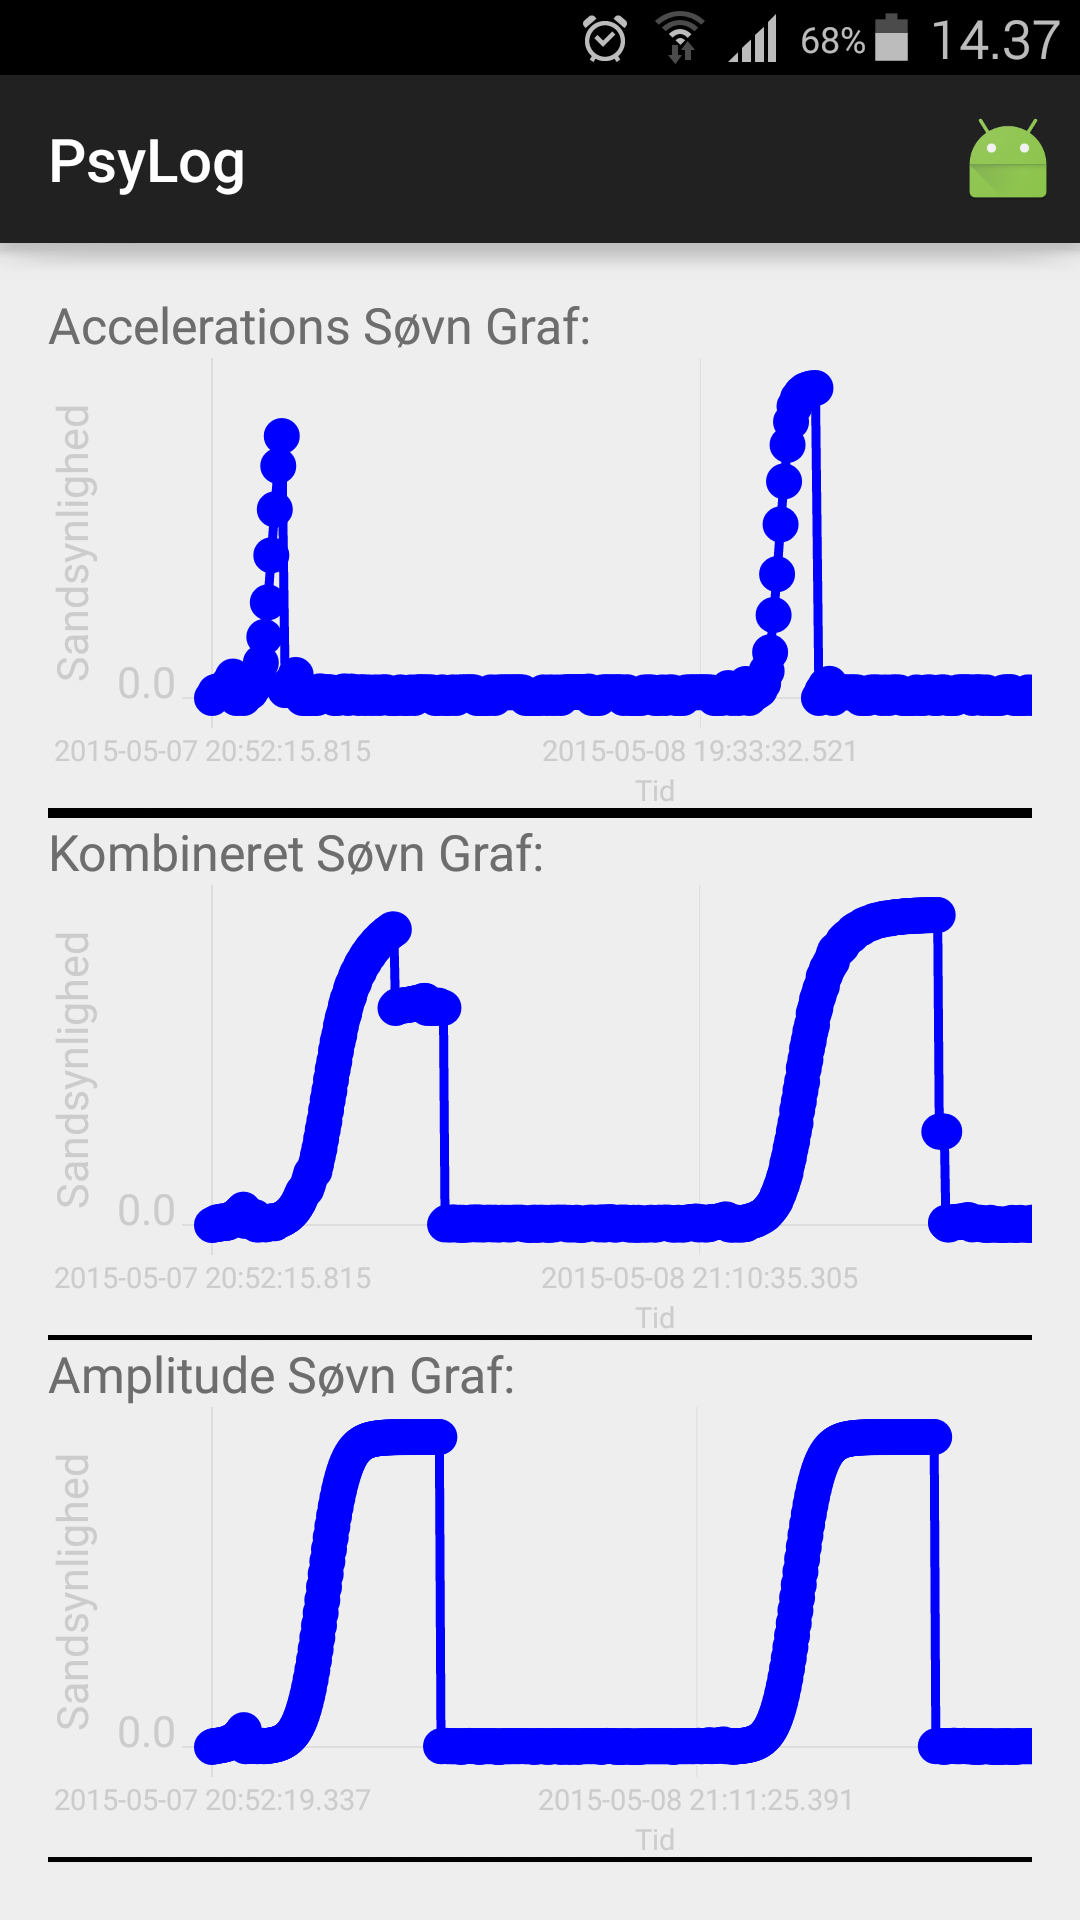
\includegraphics[scale=0.1]{visningsgrafer}
	\caption{Tre funktioner til estimering af sandsynlighed for søvn}\label{fig:visningsgrafer}
\end{figure}

Grafer er dog ikke altid lige nemme at forstå, derfor er der blevet lavet en tabel der viser hvor sikker systemet er på at man har sovet over en periode.
Denne tabel minder om den der blev vist i \cref{tab:aggdat}, dog uden $\_id$ kolonnen.
Tabellen giver et nemt overblik for brugeren om hvornår man har sovet, samt hvor sikker systemet er på at man har sovet.
Dog er det ikke så nemt for brugeren at se ens adfærdsændring i en sådan tabel, da det kræver at man kigger på meget data på en gang.

% Giv eksempel på ikke aggregeret data.
% Forklar forslag/løsning til aggregering af data.
% Vis resultat derfor
% Diskuter problemer? (e.g. snorken) evt. referer til snorken diskussion